\documentclass[UTF8]{ctexart}
\usepackage[a4paper,left=3cm,right=3cm,top=2cm]{geometry}
\usepackage{amsmath}
\usepackage{enumitem}
\usepackage{float}
\usepackage{threeparttable}
\usepackage{caption}
\usepackage{multirow}
\usepackage{graphicx}
\usepackage{listings}
\usepackage{xcolor}
\usepackage{amssymb}
\definecolor{dkgreen}{rgb}{0,0.6,0}
\definecolor{gray}{rgb}{0.5,0.5,0.5}
\definecolor{mauve}{rgb}{0.58,0,0.82}
\lstset{frame=tb,
  language=C++,
  aboveskip=3mm,
  belowskip=3mm,
  showstringspaces=false,
  columns=flexible,
  basicstyle={\small\ttfamily},
  numbers=left,%设置行号位置none不显示行号
  numberstyle=\tiny\courier, %设置行号大小
  numberstyle=\tiny\color{gray},
  keywordstyle=\color{blue},
  keywordstyle=[2]\color{purple},
  commentstyle=\color{dkgreen},
  stringstyle=\color{mauve},
  breaklines=true,
  breakatwhitespace=true,
  escapeinside=`,%逃逸字符(1左面的键),用于显示中文例如在代码中`中文...`
  tabsize=4,
  extendedchars=false %解决代码跨页时,章节标题,页眉等汉字不显示的问题
}

\iffalse
1.问题的描述
	对要解决的问题(设计目标)的详细描述,输入的数据和输出的结果。
2.算法的描述
(1)数据结构的描述
    逻辑结构和存储结构(存储类型定义、对主要变量和数组的说明)。
(2)程序结构的描述
	函数原型、功能和接口的描述。
3.调试分析
	测试数据的选择,程序调试中遇到的问题及解决方法。
4.算法的时空分析
5.测试结果及分析
	列出测试数据和测试结果,给出分析和说明。
6.实验体会和收获
\fi

\setlength\lineskiplimit{5.25bp}
\setlength\lineskip{5.25bp}

\title{实验三\ 二叉树的应用}
\author{崔士强 PB22151743}
\date{}

\begin{document}

\maketitle

\section{问题描述}
程序需要完成的操作包括:
\begin{enumerate}
  \item 输入电文字符串
  \item 统计电文字符集和每种字符在电文中出现的次数
  \item 构建 huffman 树
  \item 产生每种字符的 huffman 编码
  \item 将电文串翻译成比特流
  \item 对电文比特流进行解码
\end{enumerate}

输出信息如下所示:
\begin{table}[H]
  \centering
  \begin{tabular}{|c|c|}
    \hline
    原始字符 & 编码后字符 \\
    \hline
    aaabbbcccddd... & 一串乱码 \\
    \hline
    频率信息 & 编码信息 \\
    \hline
    a\ 5000 & a\ 1100 \\
    b\ 20000 & b\ 111 \\
    c\ 8000 & c\ 1101 \\
    d\ 4000 & d\ 0 \\
    e \ 27000 & e \ 10 \\
    ...... & ...... \\
    \hline
  \end{tabular}
\end{table}

\section{算法描述}
\subsection{数据结构描述}
本程序所用到的Huffman树存储结构如下所示:
\begin{lstlisting}
  typedef struct {
    int weight;
    int parent, lchild, rchild;
} HTNode, *HuffmanTree;

typedef char **HuffmanCode;
\end{lstlisting}
\subsection{程序结构描述}
程序中的函数声明如下:
\begin{lstlisting}
void Select(HuffmanTree HT, int n, int &s1, int &s2);
  // 在HT[1..n]中选择parent为0且weight最小的两个结点,其序号分别为s1和s2

void HuffmanCoding(HuffmanTree &HT, HuffmanCode &HC, int *weight, int n);
  // 用n个字符的权值weight构造Huffman树HT,并求出n个字符的Huffman编码HC

int ReadFile(char *filename, char *chars);
  // 从文件中逐个字节读取信息

int GetFrequency(char *chars, int *freq, char *charList, int &n);
  // 获取待处理文本字符的频率信息

void WriteCodedString(char *CodedChar, char *chars, HuffmanCode HC, char *CharList, int FLength, int CharNum);
  // 将比特流写入文件

void Decode(char *CodedChar, HuffmanCode HC, char *CharList, char *DecodedChar);
  // 根据比特流还原文件
\end{lstlisting}
\section{调试分析}
\subsection{测试数据}
选取纯文本, .mp4文件, .bmp文件, .exe文件进行测试
\subsection{问题及解决方法}
测试中发现程序无法处理除纯文本文件之外的文件类型,经调试发现数组最大值过小导致读取文件时字符频率的获取不正确。

解决方法:数组长度改为$1000000$
\section{算法的时空分析}
我们可以从以下几个方面分析复杂度:
\begin{enumerate}
  \item \lstinline{Select} 函数: 这个函数在Huffman树数组 \lstinline{HT} 中寻找两个最小的未被选中的节点。
  它通过两次遍历整个数组来实现,因此其时间复杂度为 $O(n)$。
  \item \lstinline{HuffmanCoding} 函数: 这个函数构建Huffman树。
  它首先初始化一个大小为 $2n-1$ 的数组,然后通过 $n-1$ 次迭代来构建树。
  每次迭代中,它调用 \lstinline{Select} 函数($O(n)$),然后执行常数时间的操作。
  因此,这个函数的总体时间复杂度为 $O(n^2)$。
  \item \lstinline{ReadFile} 函数: 这个函数读取文件内容。
  它的时间复杂度取决于文件的大小,假设文件大小为 $f$,则时间复杂度为 $O(f)$。
  \item \lstinline{GetFrequency} 函数: 这个函数计算每个字符的频率。
  它的时间复杂度为 $O(n^2)$,其中 $n$ 是文件内容的长度。
  \item \lstinline{WriteCodedString} 和 \lstinline{Decode} 函数: 
  这两个函数的时间复杂度取决于输入字符串的长度和字符集的大小。
  在最坏情况下,它们的时间复杂度可以达到 $O(nm)$,其中 $n$ 是输入字符串的长度,$m$ 是字符集的大小。
\end{enumerate}

这个程序的主要瓶颈在于 \lstinline{HuffmanCoding} 函数和 \lstinline{GetFrequency} 函数,
它们都有 $O(n^2)$ 的时间复杂度。
这意味着对于大型输入,这个程序的性能可能会受到显著影响。
\section{测试结果及分析}
\begin{figure}[H]
  \centering
  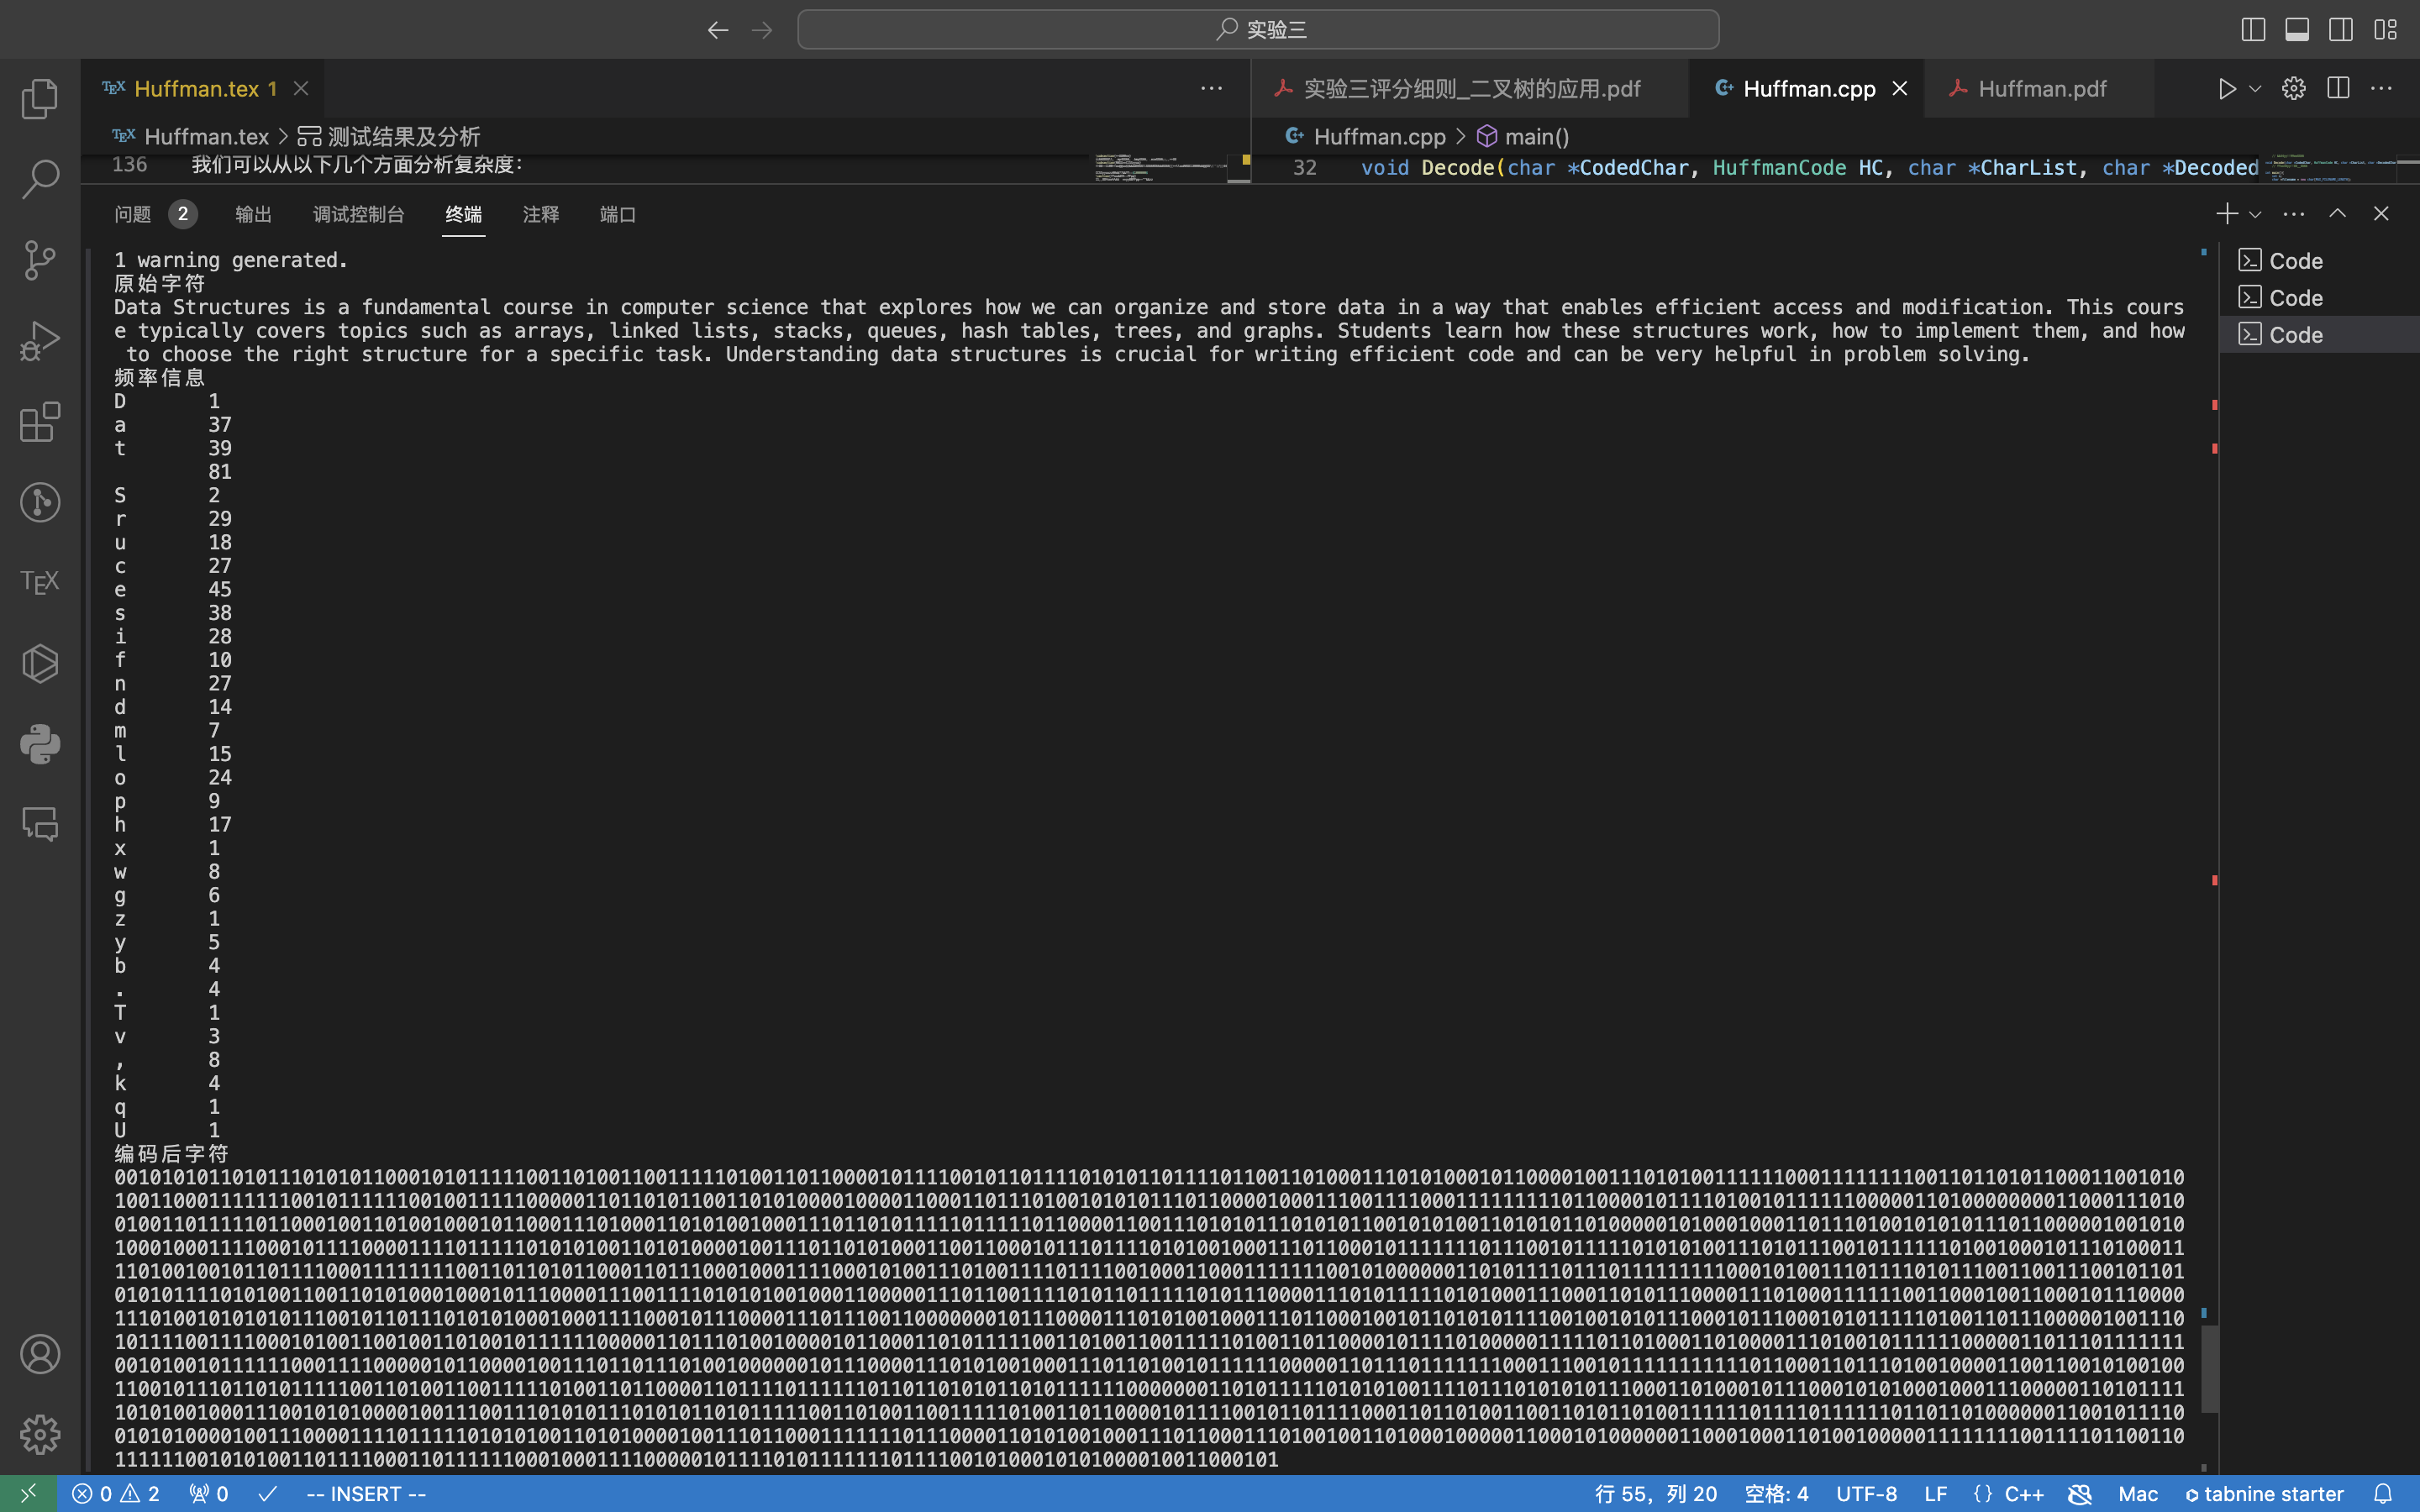
\includegraphics[scale=0.25]{test1.png}
  \caption{测试样例1}
\end{figure}
\begin{figure}[H]
  \centering
  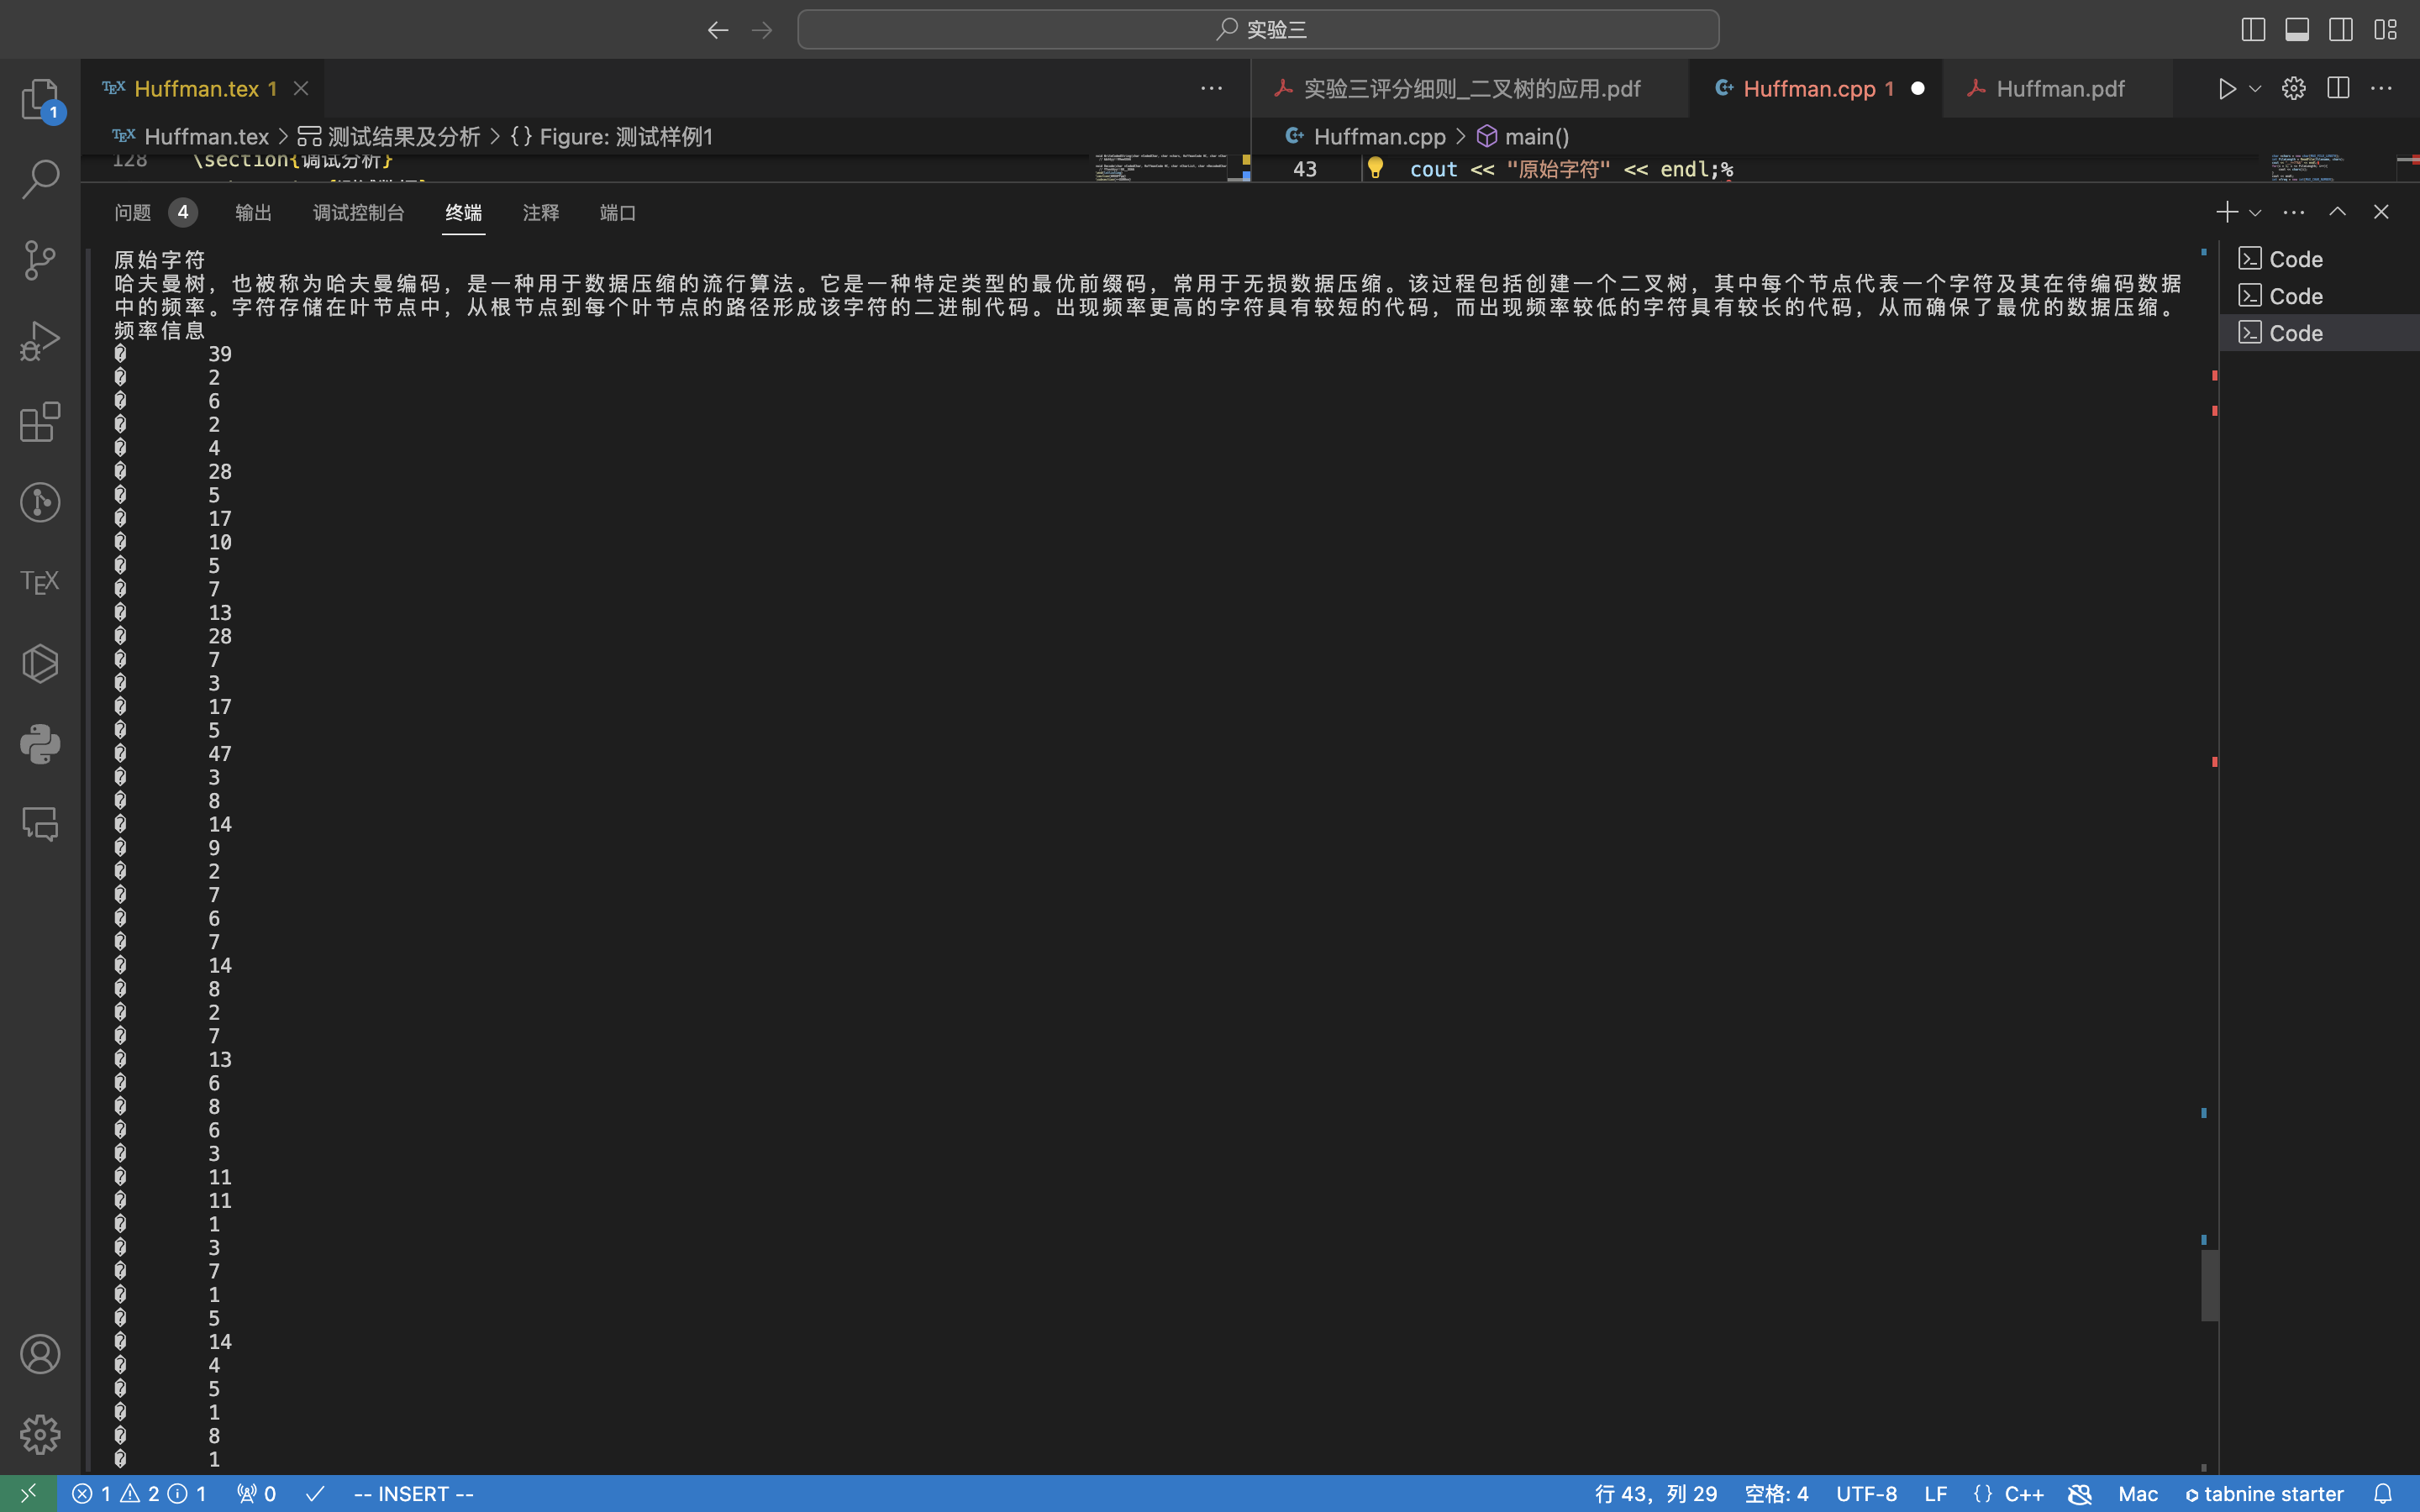
\includegraphics[scale=0.25]{test2.png}
\end{figure}
\begin{figure}[H]
  \centering
  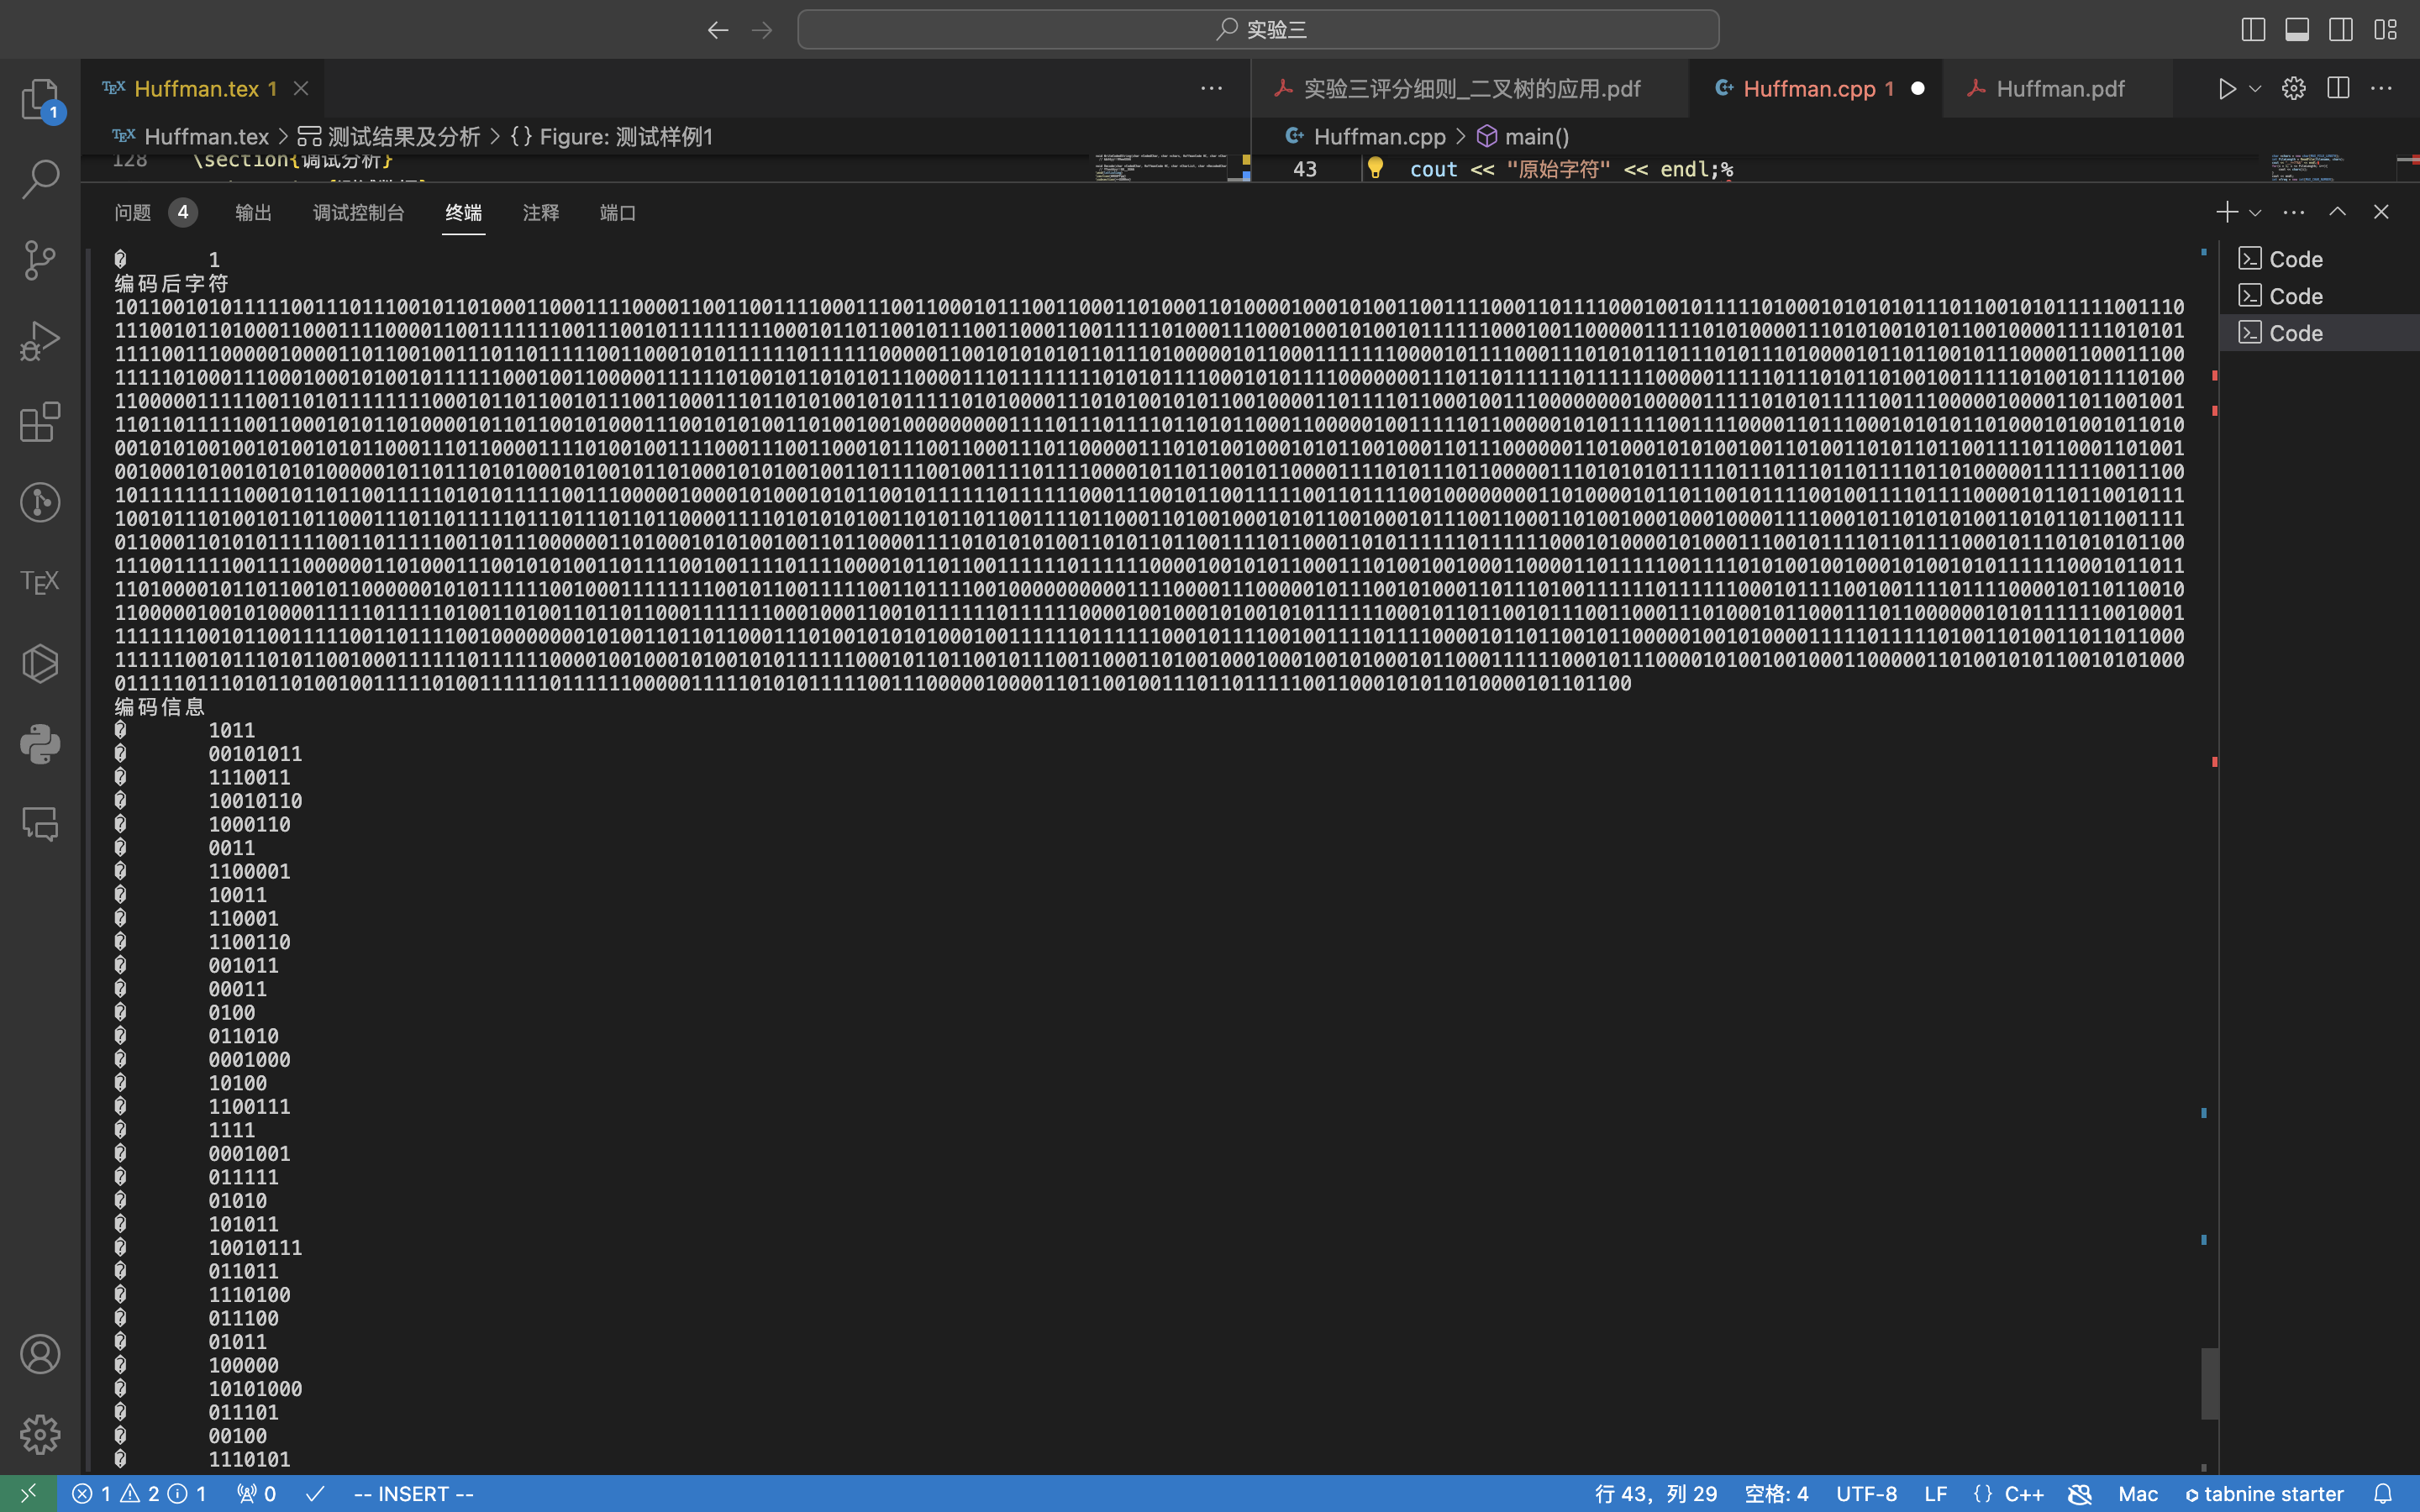
\includegraphics[scale=0.25]{test3.png}
  \caption{测试样例2}
\end{figure}
\section{实验体会和收获}
熟练掌握了二叉树的相关结构、性质,以及Huffman算法的原理。
\end{document}
